\documentclass[11pt]{article}
\usepackage[utf8]{inputenc}  % gebruik de juiste 'character encoding'
%\usepackage{a4wide}
\usepackage[english]{babel}
\usepackage{imakeidx}
\usepackage{xstring}
\usepackage{xcolor}
\definecolor{greycolour}{HTML}{525252}
\definecolor{sharelatexcolour}{HTML}{882B21}
\definecolor{mybluecolour}{HTML}{394773}
\newcommand{\wordcolour}{greycolour}

\usepackage[utf8]{inputenc}
\usepackage[
backend=bibtex,
style=numeric,
citestyle=numeric
]{biblatex}
\usepackage{amsmath} 
\usepackage{wrapfig}
\usepackage{graphicx}
\usepackage{float}
\usepackage{csquotes}
\usepackage{pdfpages}
\usepackage{listings}
\usepackage{parskip}% http://ctan.org/pkg/parskip
% https://tex.stackexchange.com/questions/55015/how-to-remove-indentation-for-all-paragraphs


\usepackage{fancyhdr}
\fancyhf{}
\rfoot{Page \thepage} 
\lfoot{Honours Team 3}
\pagestyle{fancy}

\usepackage[official]{eurosym}  % euro teken
\usepackage{subcaption}         % 2 pics
\usepackage{booktabs}           % for better tables

\graphicspath{{image/}}
\addbibresource{./Bp.bib}

\begin{document}
		\begin{center}
		\Huge Business Plan Rainbarrel\\
		 \small NS Circular Challenge
	\end{center}
	
	\begin{figure}[H]
		\centering
		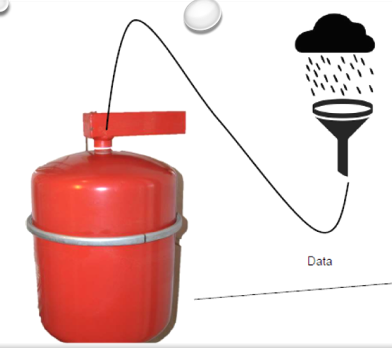
\includegraphics[width=\textwidth]{pf.png}
	\end{figure}
	
	
	\begin{table}[H]
		\begin{tabular}{l c l}
			\textbf{Name} &\textbf{Student number}& \textbf{E-mail}\\
			Timothy van der Steenhoven& 522397& 522397@student.inholland.nl \\
			Saskia van der Velden  &615128& 615128@student.inholland.nl\\
			Emmanuel Bakare &616491& 616491@student.inholland.nl\\ 
		\end{tabular}
	\end{table}
	
	\thispagestyle{empty}
	
	\newpage
	\tableofcontents
	\newpage
	
	\section*{Introduction}
	
	
	\section{Expert session 26/03/2020}
	
	\subsection{Frits \& Niels}
	Frits told us that the utilities department doesn't work until the 6th of June. The renovation has completely stopped due to the Corona crisis.
	
	Q1: What kind of doors do you have? Frits: Mostly hollow indoor-doors.
	
	After the Pitches:
	- What profit doest the rainbarrel give you?
	- Is the size enough? Why (not)?
	
	Niels: "Prove the benefit of the idea with numbers/use cases."
	
	Q2: How do you find your partners? Niels:"Get the following 3 people: The smartest guy in the room, one person with guts and someone who can manage those 2."
	
	Overall Advice: Prototype! Make it! Prove me wrong!
	
	
	\subsection{Marije Remigius}
	The Prototyping phase is iterative, meaning that you sometimes will make 15 prototypes instead of 1. There is no failure in prototyping. DIY packages?
	
	
	\section{(Re)Design}
	
	\section{Production process}
	
	\section{Finances}
	
	
	\appendix
	
	
\end{document}